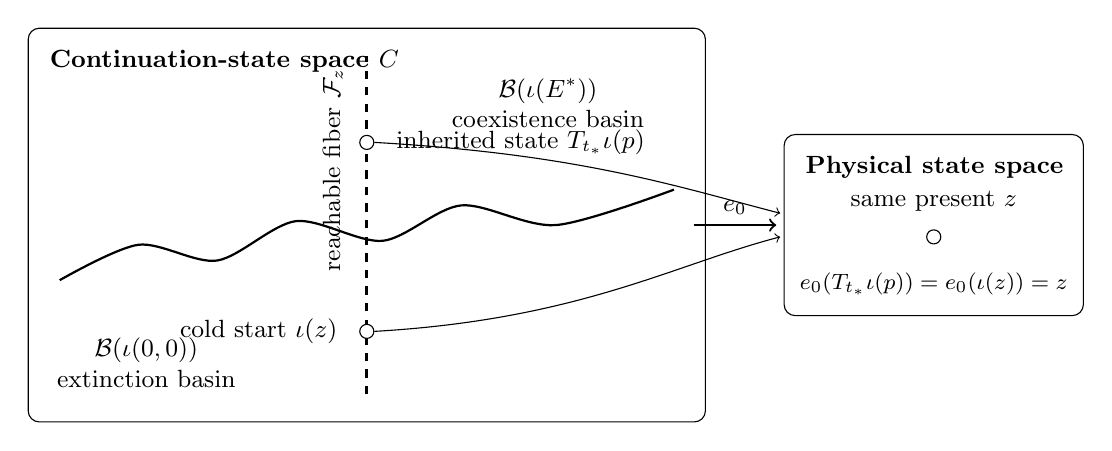
\begin{tikzpicture}[
  x=1cm,y=1cm,
  every node/.style={font=\small},
  state/.style={circle,draw,fill=white,inner sep=1.8pt},
  lab/.style={align=center}
]
  % Continuation-state space
  \draw[rounded corners] (0,0) rectangle (8.6,5.0);
  \node[anchor=north west,font=\small\bfseries] at (0.15,4.85)
    {Continuation-state space \(\mathfrak C\)};

  % Basin separator and labels
  \draw[thick] plot[smooth] coordinates {
    (0.4,1.8) (1.4,2.25) (2.4,2.05) (3.4,2.55)
    (4.5,2.30) (5.5,2.75) (6.7,2.50) (8.2,2.95)
  };
  \node[lab] at (1.5,0.75) {\(\mathcal B(\iota(0,0))\)\\extinction basin};
  \node[lab] at (6.6,4.05) {\(\mathcal B(\iota(E^*))\)\\coexistence basin};

  % Present-state fiber
  \draw[dashed,very thick] (4.3,0.35) -- (4.3,4.65);
  \node[anchor=south,rotate=90] at (4.12,3.2)
    {reachable fiber \(\mathcal F_z\)};

  % Two states in same fiber
  \node[state] (cold) at (4.3,1.15) {};
  \node[anchor=east] at (4.05,1.15)
    {cold start \(\iota(z)\)};

  \node[state] (inh) at (4.3,3.55) {};
  \node[anchor=west] at (4.55,3.55)
    {inherited state \(T_{t_*}\iota(p)\)};

  % Physical state space at right
  \draw[rounded corners] (9.6,1.35) rectangle (13.4,3.65);
  \node[anchor=north west,font=\small\bfseries] at (9.75,3.5)
    {Physical state space};
  \node[state] (z) at (11.5,2.35) {};
  \node[anchor=south] at (11.5,2.55)
    {same present \(z\)};

  % Evaluation projection
  \draw[->,thick] (8.45,2.5) -- node[above] {\(e_0\)} (9.5,2.5);
  \draw[->,thin] (inh.east) .. controls (7.0,3.4) and (8.2,3.0) .. (9.55,2.65);
  \draw[->,thin] (cold.east) .. controls (7.0,1.3) and (8.2,2.0) .. (9.55,2.35);

  % Caption-like logical statement within figure
  \node[align=center,font=\footnotesize] at (11.5,1.75)
    {\(e_0(T_{t_*}\iota(p))=e_0(\iota(z))=z\)};
\end{tikzpicture}
